\PassOptionsToPackage{dvipsnames}{xcolor}
\documentclass[fleqn,10pt]{wlscirep}

% Packages
\usepackage[super]{nth}
\usepackage{rotating}
\usepackage{makecell}
\usepackage{pifont}
\usepackage{amsfonts}
\usepackage{amsmath}
\usepackage{float}
\usepackage{pgfplots}

\pgfplotsset{compat=newest}
\usepackage{listings, textcomp}

\lstset{ %
  basicstyle=\ttfamily\footnotesize,  % size of fonts used for the code
  breaklines=true,   % automatic line breaking only at whitespace
  captionpos=b,   % sets the caption-position to bottom
  commentstyle=\color{gray},  % comment style
  keywordstyle=\color{blue},  % keyword style
  stringstyle=\color{red},  % string literal style
  upquote=true  %straight single quotes (requires textcomp)
}

\usepackage[dvipsnames]{xcolor}
\usepackage{todonotes}
\presetkeys%
    {todonotes}%
    {inline,linecolor=Plum,backgroundcolor=Plum!25,bordercolor=Plum}{}

% New Commands
\newcommand{\cmark}{\ding{51}}%
\newcommand{\xmark}{\ding{55}}%
\newcommand{\code}[1]{\texttt{#1}}

\title{SciPy 1.0---Fundamental Algorithms for Scientific Computing in Python}

\author[1]{Pauli Virtanen}
\author[2,*]{Ralf Gommers}
\author[3,4]{Tyler Reddy}
\author[5]{Anne Archibald}
\author[6]{Andrew Nelson}
\author[7]{Charles Harris}
\author[8]{CJ Carey}
\author[9]{Denis Laxalde}
\author[10]{Eric Larson}
\author[11]{Eric Moore}
\author[12]{Eric Quintero}
\author[13]{Evgeni Burovski}
\author[14]{Jaime Fernández del Río}
\author[15]{Josef Perktold}
\author[16]{Josh Wilson}
\author[17]{Matthew Brett}
\author[18]{Nikolay Mayorov}
\author[19]{Warren Weckesser}
\author[20]{Matt Haberland}
\author[21]{Scott Sievert}
\author[22]{Yu Feng}
\author[23]{Antonio Horta Ribeiro}

\affil[1]{Affiliation, department, city, postcode, country}
\affil[2]{Affiliation, department, city, postcode, country}
\affil[2]{Affiliation, department, city, postcode, country}
\affil[3]{UC Berkeley Institute for Data Science,
          Berkeley, CA, 94720, USA}
\affil[4]{Los Alamos National Laboratory,
	  Theoretical Division 6,
          Los Alamos, NM, 87545, USA}
\affil[5]{Affiliation, department, city, postcode, country}
\affil[6]{Affiliation, department, city, postcode, country}
\affil[7]{Affiliation, department, city, postcode, country}
\affil[8]{Affiliation, department, city, postcode, country}
\affil[9]{Affiliation, department, city, postcode, country}
\affil[10]{Affiliation, department, city, postcode, country}
\affil[11]{Affiliation, department, city, postcode, country}
\affil[12]{Affiliation, department, city, postcode, country}
\affil[13]{Affiliation, department, city, postcode, country}
\affil[14]{Affiliation, department, city, postcode, country}
\affil[15]{Affiliation, department, city, postcode, country}
\affil[16]{Affiliation, department, city, postcode, country}
\affil[17]{Affiliation, department, city, postcode, country}
\affil[18]{Affiliation, department, city, postcode, country}
\affil[19]{Affiliation, department, city, postcode, country}
\affil[20]{Affiliation, department, city, postcode, country}
\affil[21]{Affiliation, department, city, postcode, country}
\affil[22]{Affiliation, department, city, postcode, country}
\affil[23]{Affiliation, department, city, postcode, country}

\affil[*]{ralf.gommers@gmail.com}

\keywords{Scientific computing, Python, Mathematics}

% NOTE: some usage stats below are from https://libraries.io/pypi/scipy
% as well as github metrics; normally one doesn't put citations directly
% in abstract though (depends on field / journal)
\begin{abstract}
SciPy is an open source scientific computing library for the Python programming language.
SciPy 1.0 was released in late 2017, about 16 years after the original
version 0.1 release. SciPy
has become a \emph{de facto} standard for leveraging scientific algorithms
in the Python programming language, with more than 600
unique code contributors, millions of downloads per year, 161 dependent
packages, and 28700 dependent respositories.
The library includes functionality spanning clustering, Fourier transforms,
integration, interpolation, file I/O, linear algebra, image processing,
orthogonal distance regression, minimization algorithms, signal processing,
sparse matrix handling, computational geometry, and statistics. In this
work, we provide an overview of the capabilities and development practices of the
SciPy library and highlight some recent technical developments.
\end{abstract}
\begin{document}

\flushbottom
\maketitle
\thispagestyle{empty}

\section*{Introduction}

\textit{The Introduction section expands on the background of the work (some overlap with the Abstract is acceptable). The introduction should not include subheadings.}

\textbf{History}

\textbf{Project goals and scope}

\textbf{Current status (maturity, users)}


\section*{Architecture and implementation choices}

\subsection*{Submodule organisation}
\input{subpackages}

\subsection*{Common infrastructure}

\subsection*{Language choices}
Python, Cython, Fortran, C and C++ are the programming languages
used to implement scientific algorithms in the SciPy library. An analysis
of our code base using the \texttt{linguist} library provides a detailed
breakdown as \% composition by programming language in SciPy
(Figure~\ref{fig:linguist}).

    \begin{figure}[H]
        \centering

        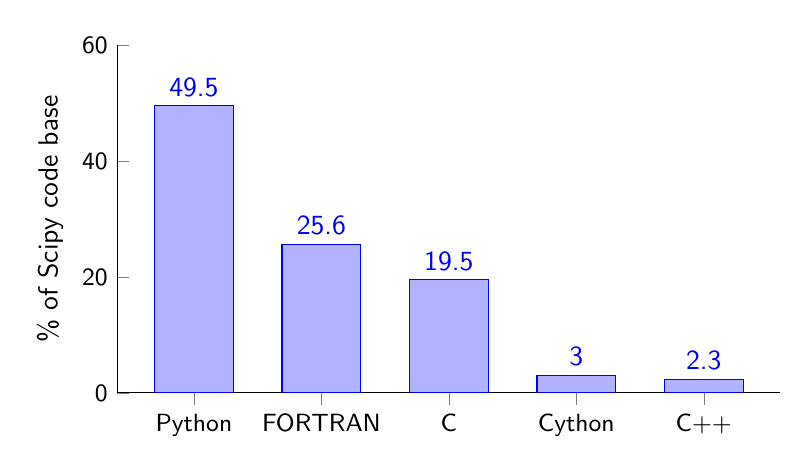
\begin{tikzpicture}[font=\sffamily]
        \begin{axis}[height=6cm, width=10cm,
        ybar, ymax=60, ymin=0,bar width=1cm,
        ylabel={\% of Scipy code base},
        ytick={0,20,...,60},
        axis lines*=left,
        axis y line shift=0pt,
        enlarge x limits=0.15,
        symbolic x coords={py,f,c,cy,cpp},
        xticklabels={Python,FORTRAN,C,Cython,C++},
        ticklabel style={align=center,font=\sffamily\small,
        /pgf/number format/assume math mode=true},
        xtick=data,
        nodes near coords,
        nodes near coords style={/pgf/number format/assume math mode=true}
        ]
        \addplot coordinates {(py,49.5) (f,25.6) (c,19.5) (cy, 3.0) (cpp,2.3)};
        \end{axis}
        \end{tikzpicture}
        \caption{The breakdown of programming languages used in the
	         SciPy library determined using the linguist library.
		 Small ($<0.5 \%$) amounts of TeX, Matlab, Shell,
		 and Makefile are excluded for clarity and mostly
		 provide supporting roles in tests, building, and
		 documentation.}
        \label{fig:linguist}
    \end{figure}

For implementing new functionality, we have a clear order of language preference.
First Python, if performance is not an issue. If it is, then in order of
preference: Cython, C, C++, Fortran. The main motivation for this is 
maintainability: Cython has the highest abstraction level and most 
Python developers will understand it. C is also widely known,
and easier to deal with for the core development team
than C++ and especially Fortran.

While it is not surprising that Python is heavily used in SciPy, the
usage distribution of the other languages warrants some discussion. Fortran
is an extremely well-established scientific programming language, both
for historical reasons and because of its continued excellent
performance\cite{Koelbel:1993:HPF:562354}. We
wrap the FFTPACK Fortran library for performing Fourier
transforms\cite{SWARZTRAUBER198445, SWARZTRAUBER198251} since
this library has been a standard in the field for 33 years and has a license
that is compatible with our own. Likewise, we wrap the Fortran source
for ODEPACK\cite{citeulike:2644528} as it has been  trusted for the initial 
value problem for ordinary differential equation systems for 30 years. For
similar reasons we also wrap the Fortran libraries QUADPACK\cite{1983qspa.book.....P} (for numerical
integration of one-dimensional functions), FITPACK\cite{Dierckx:1993:CSF:151103} (curve-fitting /
interpolation), ODRPACK\cite{ODRPACK_Boggs} (orthogonal distance regression),
MINPACK\cite{osti_6997568} (minimization of linear and nonlinear equations),
ARPACK\cite{leh:sor:yan96} (solving large scale eigenvalue problems), 
ALGORITHM 644\cite{Amos:1986:APP:7921.214331} (handling Bessel Functions), and 
CDFLIB\cite{CDFLIB_site} (evaluation of cumulative density functions).

Rounding out the top three languages in SciPy is C, which is also extremely
well-established over several decades\cite{Kernighan:1988:CPL:576122} of
scientific computing. Alongside its objected-oriented relative C++, C
can be leveraged in Python after being exposed using the Cython
language. Cython has been described as a creole language that mixes
the best parts of Python and lower-level C / C++
paradigms\cite{behnel2011cython}. We thus often use Cython as a glue
between well-established low-level scientific computing libraries and
the Python interface offered by SciPy. We also use Cython to enable
performance enhancements in Python code, especially for cases where heavily
used inner loops benefit from a compiled code with static typing. Some of the C
libraries that we wrap in SciPy include trlib\cite{doi:10.1080/10556788.2018.1449842} 
(iterative solving of the trust region problem), SuperLU\cite{li05,superlu_ug99} (solution of
large, sparse, nonsymmetric systems of linear equations),
Qhull\cite{Barber:1996:QAC:235815.235821} (computational
geometry), and Cephes\cite{cephes_netlib} (mathematics algorithms). 

Therefore, the relative abundance of different programming languages
in the SciPy library results from a combination of the usage of powerful performance
enhancing languages that interact well with Python (i.e., Cython), and
the usage of languages (and their libraries) that have proven reliable
and performant over many decades. The position that SciPy occupies
near the foundation of the scientific Python ecosystem is such that
adoption of new languages or major dependencies is generally unlikely--our
choices are strongly driven by long-term stability. GPU acceleration,
new transpiling libraries, and the latest JIT compilation approaches
(i.e., Numba\cite{Lam:2015:NLP:2833157.2833162}) are very powerful, but currently fall outside the remit
of the main SciPy library. That said, we have recently increased our
efforts to support compatibility with some of these options, and having
our full test suite pass with the PyPy JIT compiler\cite{Bolz:2009:TMP:1565824.1565827}
is now a requirement in our development workflow.

\subsection*{API and ABI evolution}
In general, we encourage changes that improve clarity in the API of the library,
but strongly discourage breaking backwards compatibility, given our position near
the base of the scientific Python computing stack.


\section*{Key technical improvements}

Here we describe key technical improvements made in the last three years.

\subsection*{Data structures}
\textbf{cKDTree}

The cKDTree module was rewritten in C++ with templated classes, and support for
periodic boundary conditions was added. A periodic boundary condition is typically 
used in computer simulations of physical processes.

% TODO: please check / improve literature citations used here
% what about the time complexity of the kNN implementation?
In 2015, we enhanced \texttt{cKDTree.query} with a $k$ nearest neighbors search
parameter. This is an efficient operation\cite{Sproull:1991:RNS:3118219.3118331} 
because it generates and returns a data structure that may be only a fraction 
of the size of the full neighbor list. A C++ implementation is provided that releases
the Python global interpreter lock for the neighbor search process, uses
a memory pool to allocate and automatically reclaim \texttt{structs}, and
heapsort to sort the $k$ nearest neighbors distances, even in the case
of periodic boundary conditions. When $k$ is a non-contiguous list of nearest
neighbors to account for (i.e., \texttt{[1, 3, 4]}), the intervening distances
between the nearest neighbor ($k = 1$) and the farthest neighbor requested
are all interrogated, but only those neighbors that are requested are retained
in memory. Thus, the maximum heap size for this algorithm is conceptually determined
as \texttt{np.arange(max(k))}.

Also in 2015, SciPy added support for generating approximated sparse distance matrices 
between \texttt{KDTree} objects (sets of points organized into a binary space 
partitioning data structure\cite{Bentley:1975:MBS:361002.361007}). 
The user provides a maximum distance value
above which all distances between points in two provided \texttt{KDTree} objects
are set to 0. The distance metric used between k-d trees is not constrained
to the conventional L2 (Euclidean) norm---any Minkowski p-norm value
bounded by 1 and infinity is valid. By default, a dictionary of keys
based sparse matrix is the returned data structure. Previously-published
results had suggested that a hashing approach to sparse matrix assembly
is 7 times faster than constructing with compressed row format (CSR)\cite{10.1007/978-3-540-75755-9_107}.
The dictionary object maps row and column indices to elements of the sparse matrix, which is
efficient for matrix construction because all zero values are skipped in
the dictionary mapping. The C++ level sparse matrix construction releases the Python
global interpreter lock for increased performance. Once constructed, the
dictionary of keys sparse matrix has the amortized constant time complexity 
($O(1)$) for distance value retrieval that one would expect from a 
dictionary\cite{Cormen:2001:IA:580470}. For efficiently performing arithmetic
operations on the sparse matrix, SciPy allows the dictionary of keys
sparse matrix to be directly converted to the common CSR, CSC, and COO
data structures.

The cKDTree module implements a dual tree counting algorithm\cite{Moore2000ar},
with an improvement to the pair counting algorithm to improve the scaling
with the number of bins. The cKDTree can now be augmented by weights, with 
weighted paircount essential in many scientific applications, e.g. computing 
correlation functions of galaxies\cite{0004-637X-750-1-38}.

\textbf{Add a Figure to show the scaling, before and after.}
\textbf{perhaps give an example or some formula.}
(cite / mention faster implementions of paircounting algorithms / treecorr, corrfunc)

The main purpose of the paircounting algorithm in cKDTree is to provide a readily
available tool. The KDTree based algorithm is not necessarily the fastest algorithm
depending on the application. E.g. for low number densities a chaining mesh based algorithm
can be easily many times faster than a tree based algorithm\cite{1991ApJ}.


\textbf{Sparse matrices}

\subsection*{Unified bindings to compiled code}
\subsubsection*{LowLevelCallable}
As of SciPy version 0.19, it is possible for users to wrap low-level
functions in a \texttt{scipy.LowLevelCallable()} object that reduces
the overhead for calling compiled C functions directly from Python.
Supported low-level functions include \texttt{PyCapsule} objects,
ctypes function pointers, and cffi function pointers. The low level
function signature must be consistent with the expectations of the
routine it is passed to. For example, the documentation for
\texttt{scipy.ndimage.generic\_filter} defines two acceptable C callback
function signatures that may be used to produce functions that operate
on each element of image data with low overhead. The C code may be
generated using numba or Cython, for example, as long as the function
call signature matches the specifications. Furthermore, it is even
possible to generate a low-level callback function automatically
from a Cython module using \texttt{scipy.LowLevelCallable.from\_cython}.

\subsection*{Cython bindings for BLAS, LAPACK and special}

\subsection*{Numerical optimization}
\newcommand{\RR}{\ensuremath{\mathbb{R}}}
The \texttt{scipy.optimize} subpackage provides functions for the numerical
solution of several classes of root finding and optimization problems.
Here we highlight recent additions through SciPy 1.0.

%\subsubsection{Root Finding}
%The general ``root finding'' problem is to find a root $\mathbf{x} \in \RR^m$ of $\mathbf{f}: \RR^m \rightarrow \RR^m$, that is, to solve
%\begin{equation}
%\mathbf{f}(\mathbf{x}) = \mathbf{0}
%\end{equation}
%for a solution $\mathbf{x}$.\footnote{Equivalently the problem is to simultaneously find the roots $x_i \in \RR$ of several scalar functions $f_i : \RR \rightarrow \RR$, that is, to solve $f_i(x_0, x_1, \dots, x_{m-1}) = 0$ for $x_i$, $i \in \{0, 1, \dots {m-1}\}$.} The function \texttt{scipy.optimize.root} provides a common interface to several algorithms for solving problems of this type. For the special case\footnote{that is, to solve a single scalar equation $f(x) = 0$ for a single scalar variable $x$} $m = 1$, any one of several specialized functions \texttt{brentq}, \texttt{brenth}, \texttt{ridder}, \texttt{bisect}, or \texttt{newton} may provide improved performance or accuracy. (Have there been any recent improvements? Do we want to summarize the methods as @antonior92 has done for $minimize$? Do we have to explain that these methods only provide \emph{one} solution, and that they are iterative based on a user-provided guess? Do we have to explain the notion of tolerance? Is this a good template for the beginning of the following subsections?)


\subsubsection*{Linear Optimization}

A new interior-point optimizer for continuous linear programming problems, \texttt{linprog} with \texttt{method='interior-point'}, was released with SciPy 1.0. Implementing the core algorithm of the commercial solver MOSEK \cite{andersen2000mosek}, it solves all of the 90+ NETLIB LP benchmark problems \cite{netlib} tested. Unlike some interior point methods, this homogeneous self-dual formulation provides certificates of infeasibility or unboundedness as appropriate. 

A presolve routine \cite{andersen1995presolving} solves trivial problems and otherwise performs problem simplifications, such as bound tightening and removal of fixed variables, and one of several routines for eliminating redundant equality constraints is automatically chosen to reduce the chance of numerical difficulties caused by singular matrices. Although the main solver implementation is pure Python, end-to-end sparse matrix support and heavy use of SciPy's compiled linear system solvers---often for the same system with multiple right hand sides due to the predictor-corrector approach---provide speed sufficient for problems with tens of thousands of variables and constraints.

Compared to the previously implemented simplex method, the new interior-point method is faster for all but the smallest problems, and is suitable for solving medium- and large-sized problems on which the existing simplex implementation fails. However, the interior point method typically returns a solution near the center of an optimal face, yet basic solutions are often preferred for sensitivity analysis and for use in mixed integer programming algorithms. This motivates the need for a crossover routine or a new implementation of the simplex method for sparse problems in a future release, either of which would require an improved sparse linear system solver with efficient support for rank-one updates.

\subsubsection*{Nonlinear Optimization}
\paragraph{Local Minimization}
The \texttt{minimize} function provides a unified interface for finding local minima of nonlinear optimization problems. A detailed comparison of the characteristics of all \texttt{minimize} methods is presented with references in Table~\ref{tab:minimize-si}. This table illustrates the level of completeness that SciPy aims for when covering a numerical method or topic.

In recent SciPy versions, four new methods for unconstrained optimization have been added to \texttt{minimize}: \texttt{dogleg}, \texttt{trust-ncg}, \texttt{trust-exact}, and \texttt{trust-krylov}. All are trust-region methods that build a local model of the objective function based on first and second derivative information, approximate the best point within a local ``trust region'', and iterate until a local minimum of the original objective function is reached, but each has unique characteristics that make it appropriate for certain types of problems. For instance, \texttt{trust-exact} achieves fast convergence by solving the trust-region subproblem almost exactly, but it requires the second derivative Hessian matrix to be stored and factored every iteration, which may preclude the solution of large problems ($\geq 1000$ variables). On the other hand, \texttt{trust-ncg} and \texttt{trust-krylov} are well-suited to large-scale optimization problems because they do not need to store and factor the Hessian explicitly, instead using second derivative information in a faster, approximate way.

\paragraph{Global Minimization}
As \texttt{minimize} may return any local minimum, some problems require the use of a global optimization routine. The new \texttt{scipy.optimize.differential\textunderscore evolution} function \cite{Wormington1999,Storn1997} is a stochastic global optimizer that works by evolving a population of candidate solutions. In each iteration, trial candidates are generated by combination of candidates from the existing population. If the trial candidates represent an improvement, then the population is updated. Most recently, the SciPy benchmark suite gained a comprehensive set of 196 global optimization problems for tracking the performance of existing solvers over time and for evaluating whether the performance of new solvers merits their inclusion in the package.

\setlength{\tabcolsep}{3pt}
\begin{table}[H]
  \centering
  \caption{Optimization methods from \texttt{minimize}, which solves problems of the form $\min_x f(x)$, where $x \in \mathbb{R}^n$ and $f: \mathbb{R}^n \rightarrow \mathbb{R}$ .  The field \textit{version added} specifies the algorithm's first appearance in SciPy. Algorithms with \textit{version added} ``0.6*'' were added in version 0.6 or before.
    The field \textit{wrapper} indicates whether the implementation available in SciPy wraps a function written in a compiled language
    (e.g. C or FORTRAN). The fields \textit{\nth{1}} and \textit{\nth{2} derivatives}
    indicates whether first or second order derivatives are required. When \textit{\nth{2} derivatives} is flagged
    with $\sim$ the algorithm does not requires second-order derivatives from
    the user; it computes an approximation internally and uses it to accelerate method convergence.
    \textit{Iterative Hessian factorization} denotes algorithms that factorize the Hessian in an iterative way,
    which does not require explicit matrix factorization or storage of the Hessian.
    \textit{Local convergence} gives a lower bound on the rate of convergence of the iterations sequence once the
    iterate is sufficiently close to the solution: linear (L), superlinear (S) and quadratic (Q). Convergence rates denoted S$^*$ indicate that the algorithm
    has a superlinear rate for the parameters used in SciPy, but can  achieve a quadratic convergence rate with other parameter choices.
    \textit{Global convergence} is marked for the algorithms with guarantees of convergence to a stationary
    point (i.e. a point $x^*$ for which $\nabla f(x^*) = 0$); this is \emph{not} a guarantee of convergence to a global minimum. The table also indicates which algorithms
    can deal with constraints on the variables. We distinguish among \textit{bound constraints} (i.e. $x^l \le x \le x^u$),
    \textit{equality constraints} (i.e. $c_{\text{eq}}(x) = 0$) and \textit{inequality constraints} (i.e. $c_{\text{ineq}}(x) \ge 0$).}
  \begin{tabular}{cccccccccccccc}
      & \rotatebox{80}{\texttt{Nelder-Mead}} & \rotatebox{80}{\texttt{Powell}} & \rotatebox{80}{\texttt{COBYLA}} & \rotatebox{80}{\texttt{CG}} & \rotatebox{80}{\texttt{BFGS}}&  \rotatebox{80}{\texttt{L-BFGS-B}} & \rotatebox{80}{\texttt{SLSQP}} & \rotatebox{80}{\texttt{TNC}} & \rotatebox{80}{\texttt{Newton-CG}} & \rotatebox{80}{\texttt{dogleg}} & \rotatebox{80}{\texttt{trust-ncg}} & \rotatebox{80}{\texttt{trust-exact}} & \rotatebox{80}{\texttt{trust-krylov}} \\
    \hline
    Version added &  0.6* &  0.6* &  0.6* &  0.6* &  0.6* &  0.6* &  0.9 &  0.6* &  0.6* & 0.13 & 0.13 & 0.19 & 1.0 \\
    \hline
    Wrapper & & & \cmark & & & \cmark & \cmark & \cmark & &  & & & \cmark \\
    \hline
    \nth{1} derivatives &  & & & \cmark  & \cmark & \cmark & \cmark & \cmark & \cmark & \cmark & \cmark & \cmark & \cmark \\
    \hline
    \nth{2} derivatives &  &  &  &  & $\sim$ & $\sim$ & $\sim$ & \cmark & \cmark & \cmark & \cmark & \cmark & \cmark \\
    \hline
    \makecell{Iterative Hessian \\
    factorization} & & & &  & & & & \cmark & \cmark &  & \cmark &  & \cmark \\
    \hline
    Local convergence& & & & L & S &  L & S & S$^*$ & S$^*$ & Q & S$^*$ & Q & S$^*$  \\
    \hline
    Global convergence & & &  &   & \cmark & \cmark & \cmark & \cmark & \cmark & \cmark & \cmark & \cmark & \cmark  \\
    \hline
    \makecell{Line-search (LS) or\\ trust-region (TR)} & Neither  & LS &  TR & LS & LS & LS & LS & LS & LS & TR & TR & TR & TR \\
    \hline
    Bound constraints &&&\cmark&&&&\cmark&\cmark&\cmark&&&& \\
    \hline
    Equality constraints &&&&&&&\cmark&&&&& \\
    \hline
    Inequality constraint &&&\cmark&&&&\cmark&&&&& \\
    \hline
    References & \cite{nelder_simplex_1965, wright_direct_1996} & \cite{powell_efficient_1964} &
      \cite{powell_direct_1994, powell_direct_1998, powell_view_2007} &
      \cite{polak_note_1969, nocedal_numerical_2006} & \cite{nocedal_numerical_2006} & \cite{byrd_limited_1995, zhu_algorithm_1997} &
      \cite{schittkowski_nonlinear_1982, schittkowski_nonlinear_1982-1, schittkowski_convergence_1983, kraft_software_1988} &
      \cite{nash_newton-type_1984} & \cite{nocedal_numerical_2006}  & 
      \cite{powell_new_1970, nocedal_numerical_2006} &  \cite{steihaug_conjugate_1983, nocedal_numerical_2006} &
      \cite{conn_trust_2000, more_computing_1983} & \cite{gould_solving_1999, lenders_trlib:_2016} \\
    \hline
  \end{tabular}
  \label{tab:minimize-si}
\end{table}





\subsection*{Statistical distributions}

%%%%%%%%%%%%%%%%%%%%%%%%%%%%%
\subsection*{Polynomial interpolators}
\input{poly}

\subsection*{Test and benchmark suite}

    \subsubsection*{Benchmark suite}

    The airspeed velocity (asv) library enables benchmarking Python packages over their lifetimes, and the performance of the SciPy
    code base was monitored with asv starting in February of 2015 (PR \#4501). In addition to ensuring that unit tests are passing (see above),
    confirming that performance generally remains constant or improves over the commit hash history of the project allows us to objectively
    measure that our code base is improving, to empower scientific applications.

    Consider the asv benchmark results shown in Figure~\ref{fig:asvbench}, spanning roughly nine years of project history. These demonstrate the gradual performance
    improvements in a nearest-neighbor search through \texttt{scipy.spatial.cKDTree.query()}, and can be run using the command:


    \texttt{python run.py run -e -s 800 --bench "\textbackslash btime\_query\textbackslash b" "02de46a546..b3ddb2c"}

    \begin{figure}[H]
        \centering
        \includegraphics[width=\textwidth]{static/asv_time_query_ckdtree}
        \caption{Airspeed velocity benchmarks for scipy.spatial.cKDTree.query() over a roughly nine year commit history time frame. The results are based on Python 2.7 performance on the master branch of the project using numpy 1.8.2 and Cython versions 0.27.3, 0.21.1, and 0.18 (for improved backward compatibility). Only the L2 (Euclidean) norm is shown here, and to improve backward compatibility and sampling of the benchmarks there was no application of toroidal topology to the KDTree (boxsize argument was ignored).}
        \label{fig:asvbench}
    \end{figure}

   Any pull request can be compared against the \texttt{master} branch with the command \texttt{asv continuous master new-feature}. This will provide a benchmark against the master branch and the branch a new feature is implemented in. More features are available in the documentation, including arguments to select which benchmarks to run.

    \subsubsection*{Test suite}
    The SciPy test suite is orchestrated by a continuous integration matrix
    that includes posix and Windows (32/64-bit) platforms managed by Travis CI and appveyor,
    respectively. Our tests cover Python versions 2.7, 3.4, 3.5, 3.6, and include
    code linting with pyflakes and pycodestyle. There are more than $13000$ unit
    tests in the test suite, which is written for usage with the pytest runner, and
    with a 76.5 \% coverage of approximately $204000$ lines
    of code holding steady for the last six months (Figure~\ref{fig:coverage}).
    Some of the historical components of the code base would still benefit from
    increased test coverage. Documentation for the code is automatically built and hosted 
    by the CircleCI service to facilitate evaluation of documentation changes / integrity.
    Our full test suite also passes with PyPy3, a just-in-time compiled version
    of the Python language.

\begin{figure}[H]
\centering
\includegraphics[width=\textwidth]{static/coverage-chart}
\caption{\% coverage of the SciPy code base by unit tests over the six
	 months preceding June 28, 2018 as reported by the \texttt{codecov}
	 service. The analysis of lines of source code covered is performed
	 automatically in our continuous integation suite using the
	 \texttt{pytest-cov} and \texttt{gcov} libraries.}
\label{fig:coverage}
\end{figure}
    


    % NOTE: is there a citation for PyPy?


\section*{Project organisation and community}

\textbf{Governance}

SciPy adopted an official Governance Document on August 3,
2017\cite{SciPyProjectGovernance}.
We have a Benevolant Dictator for Life (BDFL), Pauli Virtanen, leading the
project, following a detailed discussion of the governance model with the
community on the mailing list.  In practice, the overruling authority of the BDFL
is anticipated to be used only when the Steering Council cannot agree on a matter.
The BDFL is expected to consider any strong indications that they should step down;
although the BDFL may appoint a successor it is generally expected that the Steering
Council will be consulted on the matter.

The (currently) 18 member Steering Council is chaired by Ralf Gommers and performs a number of
tasks including nominating and voting on new Council Members, and actively
contributing to the progress of the project (could be code review but also
outreach activities, etc.). Generally, 1 year of sustained and substantial
contributions (not restricted to source code contributions) that improve
the project are the prerequiste for nomination of new Council Members. Council
Members do not get special treatment for the vast majority of the day to day
project activities (code submission / review), though it is anticipated that their
experience with the project will serve as helpful guidance in many matters.
Council Members have commit rights to the project, but will typically only
incorporate changes when there are no substantive community objections. The
Chair of the Steering Council is responsible for starting more formal
technical reviews of the direction of the project, ensuring that the
composition of the Council remains current, and communicating / summarizing
any Council activities performed privately to the broader community. We also
describe in some detail how institutional partners may contribute to the
project, but no financial weight from grants or other sources
may be leveraged to circumvent or overrule the technical direction of the
project decided upon by the Steering Committee. The Chair does not have
a fixed term, but is nominated by the Steering Committee and is expected
to yield to substantive claims that stepping down is the appropriate action.

SciPy adopted an official Code of Conduct on October 24, 2017
\cite{SciPyCodeOfConduct}, drawing
inspiration from the Apache Foundation Code of
Conduct\cite{ApacheCodeOfConduct}, the Contributor Covenant
\cite{ContributorConvenant},
the Jupyter Code of Conduct \cite{Jupyter_COC}, and the Open Source Guides -
Code of Conduct\cite{OSG_COC}. In short,
we stated five specific guidelines: \emph{be open} (to anyone participating in our community),
\emph{be empathetic and patient} (in resolving conflicts), \emph{be collaborative} (we depend
on each other to build up the tools in the library), \emph{be inquisitive} (identifying issues
early on can be helpful to everyone), and \emph{be careful with wording} (do not harass or exclude).
We outlined a broad diversity inclusion statement, and provide
instructions for contacting the three members of our Code of Conduct Committee or an
external representative on the NumFOCUS Board of Directors.

\textbf{Roadmap}

The SciPy Roadmap\cite{SciPy_roadmap} is a continuously-updated document
maintained by the community that describes some of the major directions
for improvement for the project, as well as specific limitations and
matters that require assistance moving forward.

We are still striving to increase the number of SciPy usage tutorials beyond
our current 15 section offering\cite{SciPy_tutorials}, but our
standard documentation for library features is already in excellent shape.


The low-level Cython code in our library (which interacts with C-level
code and exposes it for Python usage) could use some measure of modernization,
including migration to typed memoryviews to handle NumPy arrays instead of
the older syntax:

\begin{lstlisting}[language=Python]
# example of a function that takes a single
# 3 dimensional typed memoryview as an argument
# this allows Cython-level handling of a NumPy
# array object
cpdef int func_new(int[:, :, :] arr):
    pass

# example of the old syntax for handling
# the same scenario
cpdef int func_old(object[int, ndim=3, mode='strided'] arr):
    pass

\end{lstlisting}

\texttt{fftpack} and {linalg} have too much functionality overlap with
\texttt{numpy} equivalents.

\texttt{scipy.interpolate} could benefit from a set of new features including
spline fitting routines with better user control; arithmetic routines for splines;
transparent tensor-product splines, Non-Uniform Rational B-Splines support;
and mesh refinement and coarsening of B-splines and corresponding tensor products.
Some spline functionality in \texttt{scipy.signal} should be migrated to \texttt{interpolate} 
and Second Order Sections need to be updated to match the capabilities in other routines.

For \texttt{scipy.linalg}, the major change needed is to support a more recent
version of LAPACK. Users should be able access an increasing repertoire of
LAPACK functions using either \texttt{get\_lapack\_funcs} or
\texttt{sp.linalg.lapack.name\_of\_function}.

\texttt{scipy.optimize} would benefit from a few more good global optimizers 
as well as large-scale optimizers.

\texttt{scipy.ndimage} should be completely migrated to a data point
model (values on a grid), instead of a pixel model (elements with centers),
both of which have been used in the past, because the data point model is now
proving more effective in practice.

While \texttt{scipy.sparse} is mature, there are many data
formats and the community continues to move forward here so we will aim
to take advantage of their improvements\cite{abbasi2018sparse} 
while preserving backwards compatibility to the extent that it is possible.
\texttt{sparse.linalg} may benefit from wrappers for PROPACK 
for faster sparse SVD computation.

\texttt{scipy.spatial} will benefit from \texttt{spatial.transforms} with
support for rotation matrices.

\texttt{scipy.special} needs precision improvements for hypergeometric 
functions, parabolic cylinder functions, and spheroidal wave functions.




\textbf{Community beyond the SciPy library}

\textbf{Maintainers and contributors}


\section*{Discussion}

\textit{The Discussion should be succinct and must not contain subheadings.}

\textbf{Impact now}
SciPy has a strong developer community and a massive user base. GitHub
traffic metrics report roughly 20,000 unique visitors to the source
website between May 14 and May 27, 2018, with 721 unique copies (``clones")
of the code base over that roughly two-week period. The developer community
consists of 610 unique contributors of source code, with $>19,000$ commits
accepted into the code base (GitHub page data).

% need some better usage stats sources?
%
% note: @stefanv has pypinfo set up, so can grab all the info shown at
% https://github.com/ofek/pypinfo
%
% SciPy stuff from njs blog: https://docs.google.com/spreadsheets/d/1lOLvSF0up4eZyv2ugZi-TM_GIs3gPCkGNIDKXS1Y3w4/edit#gid=406031940
From the user side, there have been at least 15 million downloads
of the SciPy manylinux wheels between the start of 2016 and May of 2018
(njs blog). The recommended source for citing SciPy is simply a reference
to the website / library itself\cite{SciPylib}, and has been cited $>3000$
times. Some of the most prominent citing articles include the IPython
publication\cite{PER-GRA:2007}, a heavily-cited Nature Biotechnology
article\cite{pmid17287757}, a dark
matter annihilitation study in the field of
cosmology\cite{1475-7516-2012-08-007}, and many of the
other major downstream software libraries in the Python scientific
computing stack.

\textbf{Future development}.
Future development plans include a major rewrite of the \texttt{scipy.sparse} module, which is already underway\cite{abbasi2018sparse}. This is due to the current interface only supporting two-dimensional objects. Even sub-arrays are two-dimensional, and dimensions greater than two aren't supported. The new package supports dimensions greater than two, and it bases itself around arrays rather than matrices (which is strictly more powerful). It also features improved inter-operability with NumPy and other community packages.

\textit{This section should include key issues: sparse arrays, ndimage pixel vs point, splines, fftpack vs. np.fft and linalg vs. np.linalg, under-maintained submodules.}

\subsection*{ndimage pixel vs point}

\begin{itemize}
  \item A pixel is not a little square
    (http://alvyray.com/Memos/CG/Microsoft/6\_pixel.pdf)
  \item Match edges vs match centers
    (http://entropymine.com/imageworsener/matching/)
\end{itemize}

There are two competing models for representing image measurements:
the first considers an image as a collection of pixels, square blocks
of size 1x1 with centers offset by (0.5, 0.5).  This model corresponds
closely with a camera sensor, that integrates light as it falls on
(more-or-less) square elements, producing a digital readout for each.

Another view is that of an image as a grid of point measurements.
This model explicitly rejects two notions encouraged by the pixel
model: that our signal is best represented as a step-wise function, and
that a single measurement represents knowledge of the surrounding
square area element.  Instead, we think of the image as a smoothly
varying function, of which we have measurements at grid positions.

While the representations may not seem very different, they have
significant implications for image processing algorithms such as
rescaling.

{\tt ndimage} currently follows the pixel model for operations like
{\tt zoom} but the data point model for general geometric
transformations and interpolation.  We think that consistently using
the data point model will serve us better in the long run:

\begin{enumerate}
  \item It makes no assumption about the sampling mechanism used
    (camera, scanner, laser, etc.).
  \item NumPy coordinates map directly to measurement coordinates,
    without a 0.5 offset. \todo{Will have to rethink this statement,
      since this {\bf is} the current underlying model for interpolation}
  \item It makes it easier to reason about extrapolation.  E.g., the current
    dubious notion of ``reflection'', in which the image is padded
    {\tt d c b a | a b c d | d c b a} becomes nonsensical, and leaves
    only the reliable notion of mirroring, {\tt d c b | a b c d | c b a}.
\end{enumerate}

The second model, while consistent, does introduce some challenges
w.r.t. traditional image manipulation (see attached figure).

\begin{figure}[H]
    \centering
    \includegraphics[width=0.5\textwidth]{static/image_pixel_model}
    \caption{Upscaling an image 2x.  In the data point model, the
      original data points remain in the image corners, which means it
      contributes less to the center of the resulting image than to
      the corners.  In the pixel model, the original pixels contribute
      more evenly to both of these.}
    \label{fig:image-pixel-model}
\end{figure}

\bibliography{references}

\noindent Use the cite command for an inline citation, e.g. \cite{behnel2011cython}.

\section*{Acknowledgements (not compulsory)}

Acknowledgements should be brief, and should not include thanks to anonymous referees and editors, or effusive comments. Grant or contribution numbers may be acknowledged.

\section*{Author contributions statement}

Must include all authors, identified by initials, for example:
A.A. conceived the experiment(s),  A.A. and B.A. conducted the experiment(s), C.A. and D.A. analysed the results.  All authors reviewed the manuscript.

\section*{Additional information}

To include, in this order: \textbf{Accession codes} (where applicable); \textbf{Competing financial interests} (mandatory statement).

The corresponding author is responsible for submitting a \href{http://www.nature.com/srep/policies/index.html#competing}{competing financial interests statement} on behalf of all authors of the paper. This statement must be included in the submitted article file.

\end{document}

%%% Local Variables:
%%% mode: latex
%%% TeX-master: t
%%% End:
